\documentclass[18pt]{beamer}
\usepackage{templates/beamerthemekit}
\usepackage[export]{adjustbox}
\usepackage{tikz}
\usepackage{url}
\usepackage{amsmath}
\usepackage{marvosym} % \MVRIGHTarrow
\usepackage{stmaryrd} % \shortrightarrow
\usepackage{textcomp} % \textrightarrow
\usepackage{svg}

\title[Progress Update]{Towards Bringing Together Numerical Methods for Partial Differential Equation and Deep Neural Networks}
\subtitle{Progress Update, Supervisor - Markus Hoffmann}
\author{Stanislav Arnaudov}
\institute{Chair for Computer Architecture and Parallel Processing}
\date{September 26, 2019}
\selectlanguage{english}

% \usepackage[style=verbose,backend=bibtex]{biblatex}
% \bibliography{bib}
% \bibliographystyle{plain}

% \newcommand{\semitransp}[2][35]{\color{fg!#1}#2 \color{fg}}

\begin{document}

\begin{frame}
 \titlepage
\end{frame}

\section{Description}

\begin{frame}[t]
  \frametitle{Project description}
  \begin{center}
    \large{\textbf{Basic idea:} Perform numerical simulation with ML-models}
  \end{center}
\end{frame}


\begin{frame}[t]
  \frametitle{Project description}
  \begin{center}
    \large{\textbf{Basic idea:} Perform numerical simulation with ML-models}
  \end{center}
  
  \begin{itemize}
  \item Concrete problem: Flow around an object according to the Navier–Stokes equations.
  \end{itemize}

  \begin{figure}[htb]
    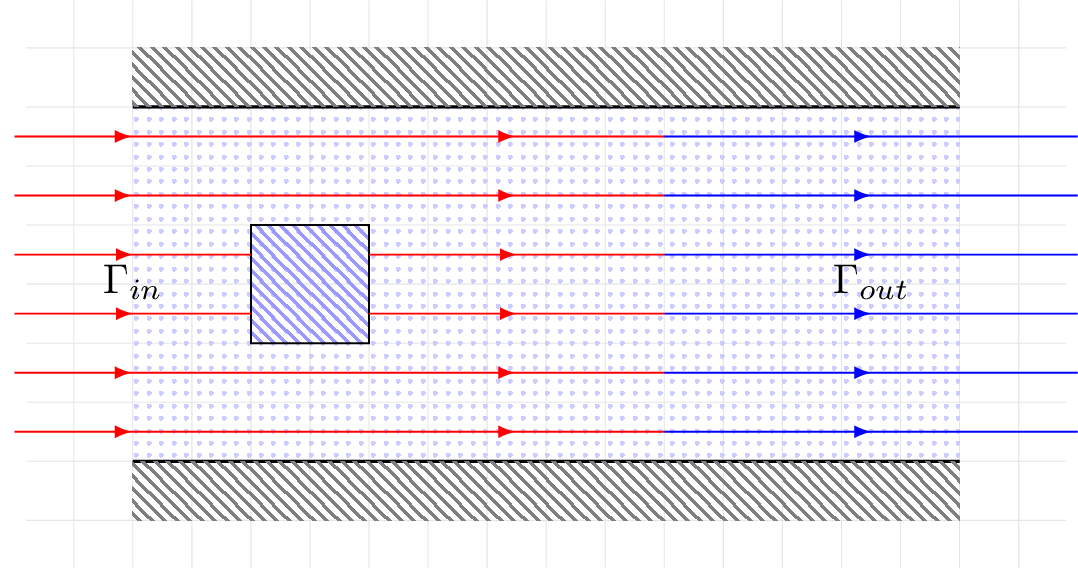
\includegraphics[scale=0.24]{images/channel/flow_2}
    \caption{Simulation Setup}
  \end{figure}
  
\end{frame}

\begin{frame}[t]
  \frametitle{Project description}
  \begin{center}
    \large{\textbf{Basic idea:} Perform numerical simulation with ML-models}
  \end{center}
  \begin{itemize}
  \item Solutions of the simulation can be represented as images.
  \end{itemize}

  \begin{figure}[htb]
    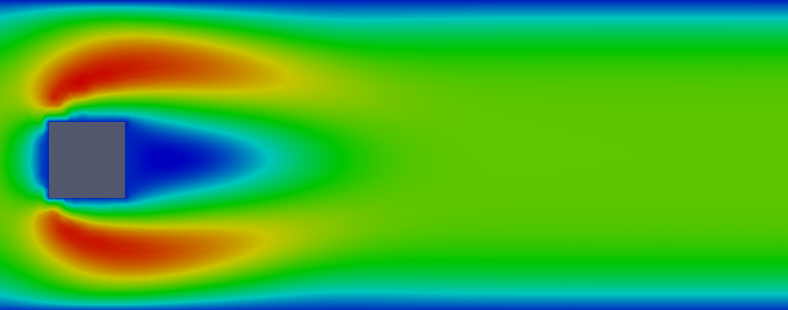
\includegraphics[scale=0.38]{images/flow_solution}
    \caption{Simulation Image}
  \end{figure}

  
\end{frame}


\begin{frame}[t]
  \frametitle{Project description}
  \begin{center}
    \large{\textbf{Basic idea:} Perform numerical simulation with ML-models}
  \end{center}
  
  \begin{itemize}
  \item Or ML-model primarily use images as input and output.
  \end{itemize}

  \begin{center}
    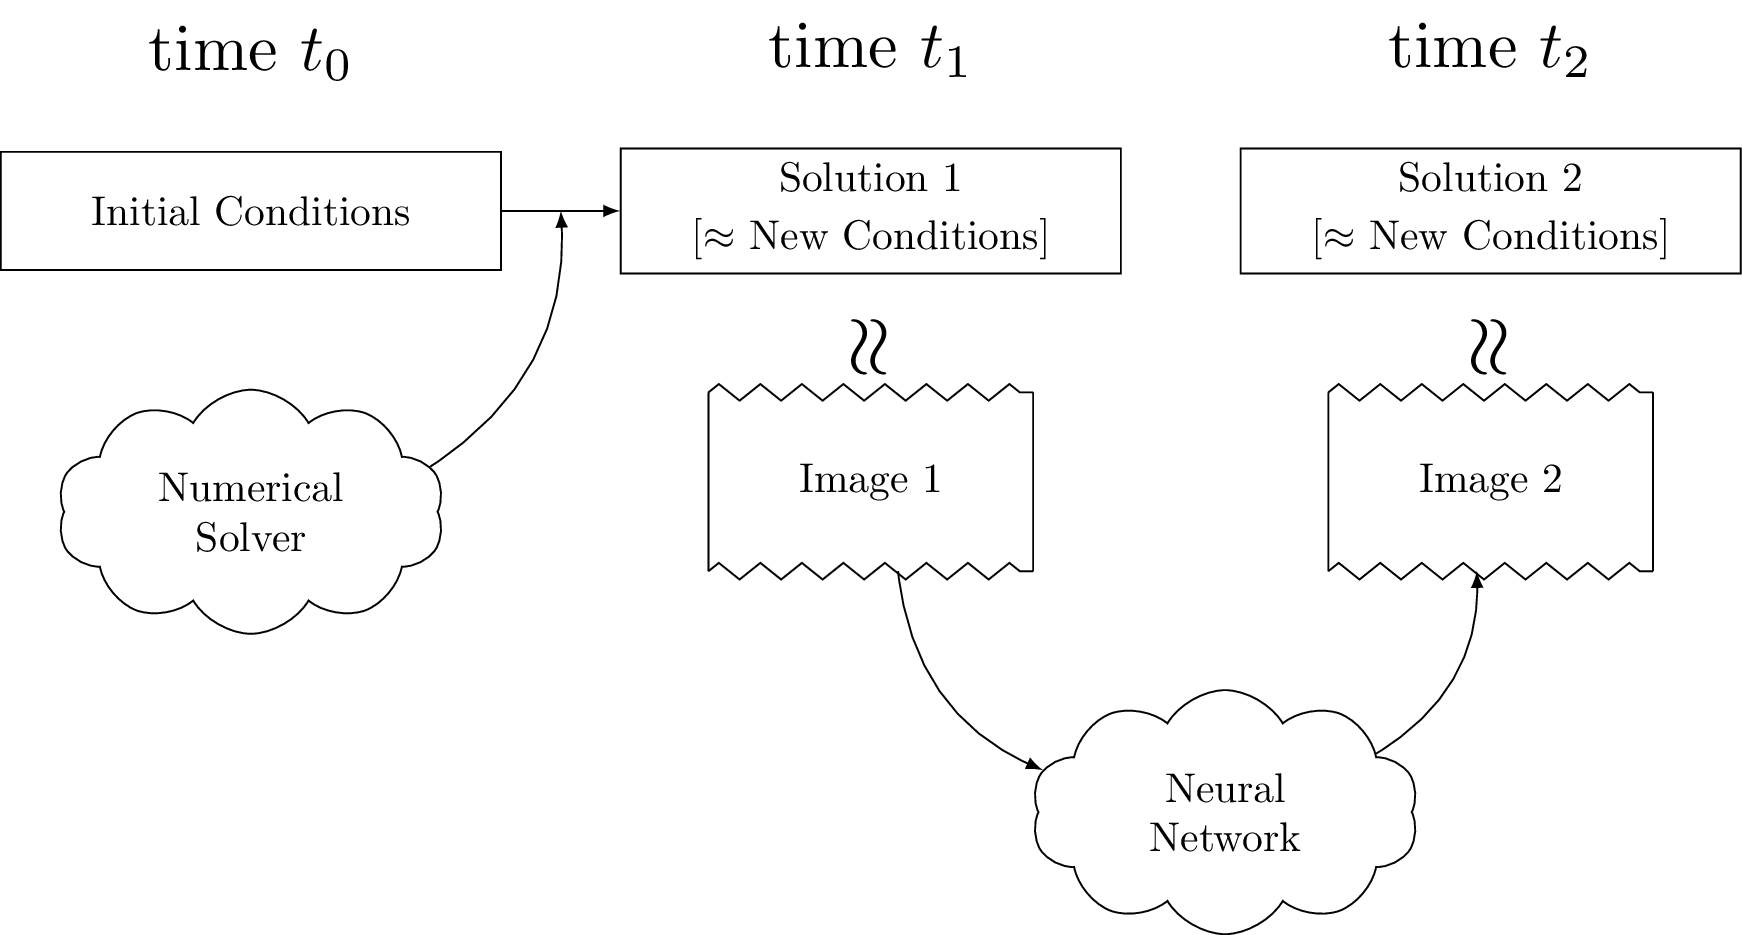
\includegraphics[scale=0.15]{images/new/overview}
  \end{center}
  
\end{frame}

\begin{frame}[t]
  \frametitle{Project description}
  \large{Several cases to investigate}
  \begin{itemize}
  \item Constant model
  \item Fluid speed model
  \item Fluid viscosity and density model
  \item Object in space model
  \end{itemize}
  
% system overview here
\end{frame}

\section{Data}
\begin{frame}[t]
  \frametitle{Data Generation}
  \begin{itemize}
  \item Use of numerical solver for real simulation data generation.
  \item The simulation has several adjustable parameters
    \begin{itemize}
    \item inflow speed
    \item fluid viscosity
    \item fluid density
    \end{itemize}
  \item Reynolds Number in the range of [90, 350]
  \end{itemize}  
\end{frame}

\begin{frame}[t]
  \frametitle{Data Generation}
  \begin{itemize}
  \item Use of numerical solver for real simulation data generation.
  \item The simulation has several adjustable parameters
  \item Reynolds Number in the range of [90, 350]
  \end{itemize}
\end{frame}


\begin{frame}[t]
  \frametitle{Data Generation}
  \begin{itemize}
  \item Use of numerical solver for real simulation data generation.
  \item The simulation has several adjustable parameters
  \item Reynolds Number in the range of [90, 350]
  \end{itemize}
  % karman vortex street here
  \begin{center}
    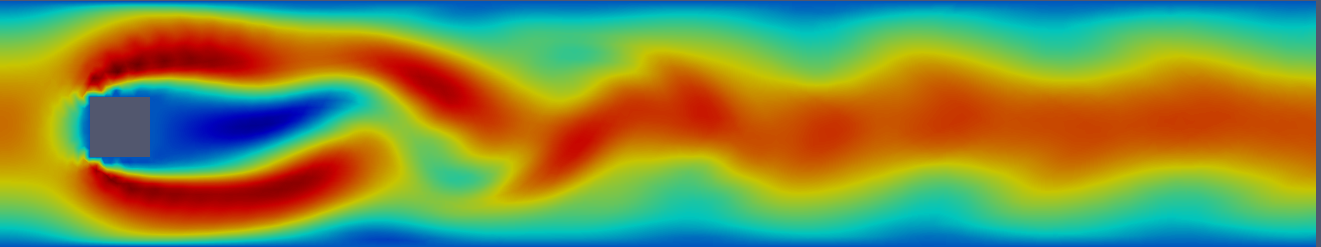
\includegraphics[scale=0.21]{images/x-direction}
  \end{center}
  \begin{center}
    \begin{figure}[htb]
    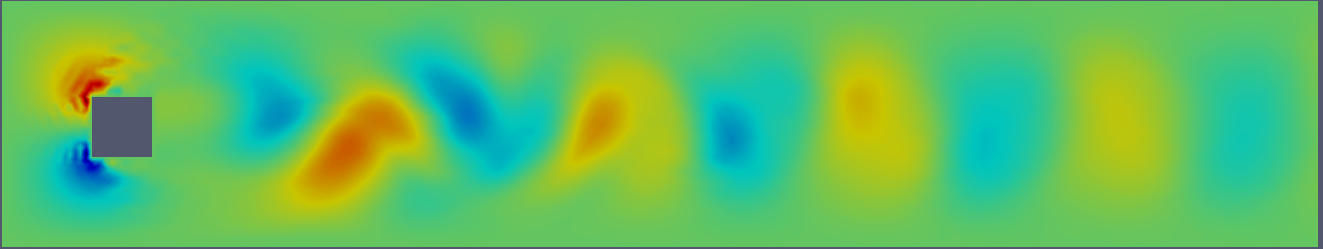
\includegraphics[scale=0.21]{images/y-direction} \\
    \caption{Karman vortex street}
    \end{figure}
  \end{center}
\end{frame}

\begin{frame}[t]
  \frametitle{Data Generation}
  \begin{itemize}
  \item Use of numerical solver for real simulation data generation.
  \item The simulation has several adjustable parameters
  \item Reynolds Number in the range of [90, 350]
  \item Choosing appropriate color space : Grayscale or RGB
  \end{itemize}

  \begin{center}
    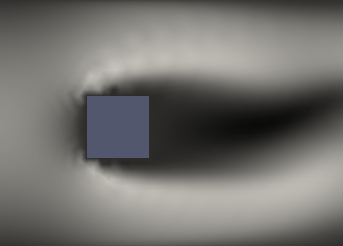
\includegraphics[scale=0.27]{images/x-direction-gray} \hspace{0.7cm}
    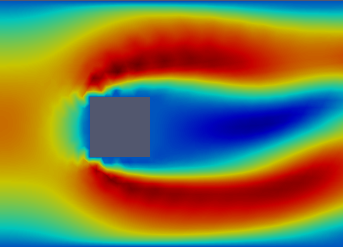
\includegraphics[scale=0.27]{images/x-direction-rgb} \\ \vspace{0.2cm}
    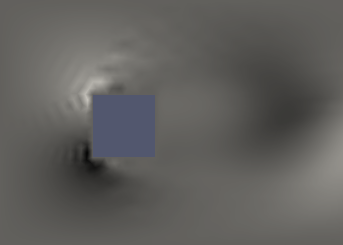
\includegraphics[scale=0.27]{images/y-direction-gray} \hspace{0.7cm}
    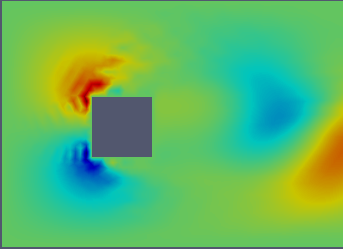
\includegraphics[scale=0.27]{images/y-direction-rgb} \\
  \end{center}
  
\end{frame}

\section{Models}
\begin{frame}[t]
  \frametitle{Models}
  \begin{itemize}
  \item Two types of architectures based on our preliminary research:
  \end{itemize}
\end{frame}


\begin{frame}[t]
  \frametitle{Models}
  \begin{itemize}
  \item Two types of architectures based on our preliminary research:
    \begin{itemize}
    \item ResNet 
    \end{itemize}
  \end{itemize}

  \vspace{1cm}
  \begin{center}
      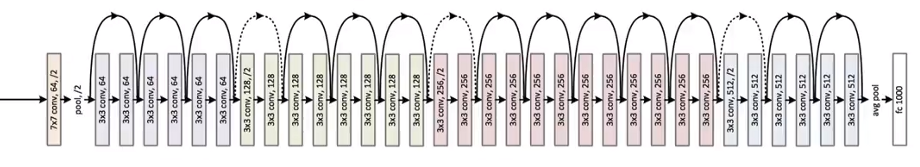
\includegraphics[scale=0.37]{images/nets/res}
    \end{center}
\end{frame}


\begin{frame}[t]
  \frametitle{Models}
  \begin{itemize}
  \item Two types of architectures based on our preliminary research:
    \begin{itemize}
    \item UNet
    \end{itemize}
  \end{itemize}

  \vspace{1cm}
  \begin{center}
    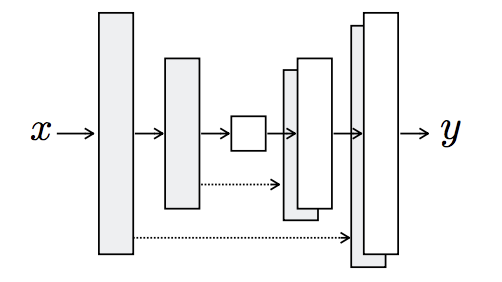
\includegraphics[scale=0.37]{images/nets/unet}
  \end{center}
  
\end{frame}


\begin{frame}[t]
  \frametitle{Models}
  \begin{itemize}
  \item Two types of architectures based on our preliminary research:
    \begin{itemize}
    \item UNet turned out to perform better.
    \end{itemize}
  \end{itemize}
\end{frame}


\begin{frame}[t]
  \frametitle{Models}
  \begin{itemize}
  \item Two types of architectures based on our preliminary research:
  \item Data being used by the network.
  \end{itemize}
\end{frame}

\begin{frame}[t]
  \frametitle{Models}
  \begin{itemize}
  \item Two types of architectures based on our preliminary research:
  \item Data being used by the network.
    \begin{itemize}
    \item Usage of pressure field
    \end{itemize}
  \end{itemize}

  \vspace{0.5cm}
  \begin{center}
    \includegraphics[scale=0.20]{images/models/pressure_optional}
  \end{center}  
\end{frame}


\begin{frame}[t]
  \frametitle{Models}
  \begin{itemize}
  \item Two types of architectures based on our preliminary research:
  \item Data being used by the network.
    \begin{itemize}
      \item Usage of pressure field $\rightarrow$ the pressure field turned out to be useful
    \end{itemize}
  \end{itemize}

  \vspace{0.5cm}
  \begin{center}
    \includegraphics[scale=0.20]{images/models/pressure_optional}
  \end{center}  
\end{frame}

\begin{frame}[t]
  \frametitle{Models}
  \begin{itemize}
  \item Two types of architectures based on our preliminary research:
  \item Data being used by the network.
    \begin{itemize}
    \item Processing of real values
    \end{itemize}
  \end{itemize}

  \vspace{0.5cm}
    \begin{center}
    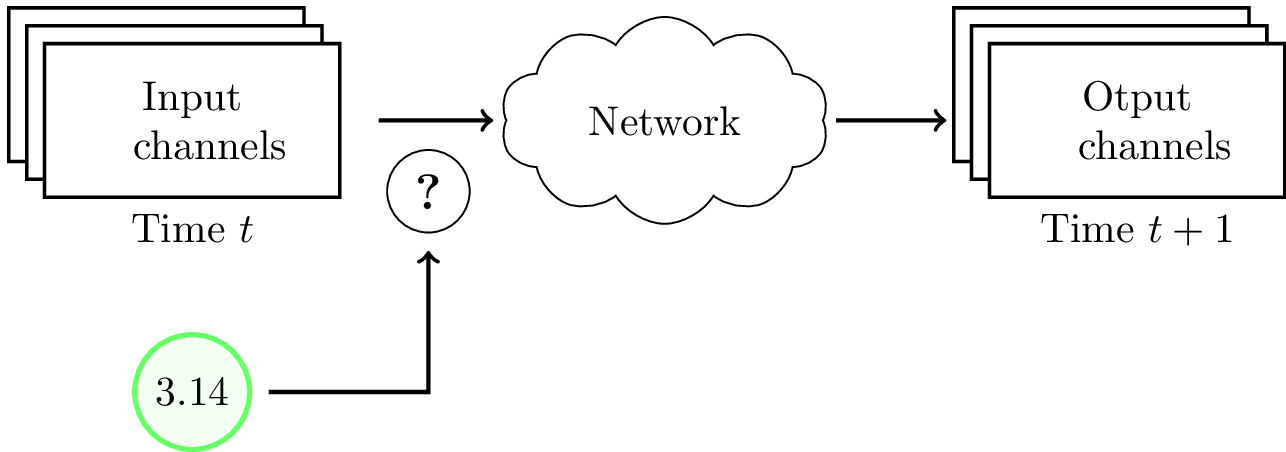
\includegraphics[scale=0.20]{images/models/num_question}
  \end{center}
\end{frame}


\begin{frame}[t]
  \frametitle{Models}
  \begin{itemize}
  \item Two types of architectures based on our preliminary research:
  \item Data being used by the network.
    \begin{itemize}
    \item Processing of real values $\rightarrow$ extra image channel filled with the value
    \end{itemize}
  \end{itemize}

  \vspace{0.3cm}
    \begin{center}
    \includegraphics[scale=0.20]{images/models/num_answer}
  \end{center}
  
\end{frame}

\section{Evaluation}

\begin{frame}
  \frametitle{Evaluating the results}
\end{frame}

\begin{frame}[t]
  \frametitle{Evaluating the results}
  \begin{center}
    \textbf{\Large Two views of the results}
  \end{center}
  \vspace{-1cm}
  \begin{columns}[t]
    \begin{column}{0.5\textwidth}
      \begin{center}
        {\large \underline{Computer Vision}}
      \end{center}
    \end{column}
    \begin{column}{0.5\textwidth}
      \begin{center}
        {\large \underline{Numerical Simulation}}
      \end{center}  
    \end{column}
  \end{columns}
\end{frame}


\begin{frame}[t]
  \frametitle{Evaluating the results}
  \begin{center}
    \textbf{\Large Two views of the results}
  \end{center}
  \vspace{-1cm}
  \begin{columns}[t]
    \begin{column}{0.5\textwidth}
      \begin{center}
        {\large \underline{Computer Vision}}
        \begin{itemize}
        \item Perceived qualities of the \underline{image} results
        \item Metrics:
          \begin{itemize}
          \item Peak signal-to-noise ratio - PSNR
          \item Correlation
          \end{itemize}
        \end{itemize}
      \end{center}
    \end{column}
    \begin{column}{0.5\textwidth}
      \begin{center}
        {\large \underline{Numerical Simulation}}
      \end{center}  
    \end{column}
  \end{columns}
\end{frame}


\begin{frame}[t]
  \frametitle{Evaluating the results}
  \begin{center}
    \textbf{\Large Two views of the results}
  \end{center}
  \vspace{-1cm}
  \begin{columns}[t]
    \begin{column}{0.5\textwidth}
      \begin{center}
        {\large \underline{Computer Vision}}
        \begin{itemize}
        \item Perceived qualities of the \underline{image} results
        \item Metrics:
          \begin{itemize}
          \item Peak signal-to-noise ratio - PSNR
          \item Correlation
          \end{itemize}
        \end{itemize}
      \end{center}
    \end{column}
    \begin{column}{0.5\textwidth}
      \begin{center}
        {\large \underline{Numerical Simulation}}
        \begin{itemize}
        \item \underline{Real} differences between the predicted and the actual \underline{values}
        \item Metrics:
          \begin{itemize}
            \item Average percentage difference
            \item Max percentage difference
          \end{itemize}
        \end{itemize}
      \end{center}  
    \end{column}
  \end{columns}
\end{frame}


\begin{frame}[t]
  \frametitle{Evaluation cases}
  \begin{center}
    \textbf{\Large Two evaluation cases}
  \end{center}
  \vspace{-1cm}
  \begin{columns}[t]
    \begin{column}{0.5\textwidth}
      \begin{center}
        {\large \underline{Individual Images}}
      \end{center}
    \end{column}
    \begin{column}{0.5\textwidth}
      \begin{center}
        {\large \underline{Recursive Application}}
        \end{center}
    \end{column}
  \end{columns}
\end{frame}


\begin{frame}[t]
  \frametitle{Evaluation cases}
  \begin{center}
    \textbf{\Large Two evaluation cases}
  \end{center}
  \vspace{-1cm}
  \begin{columns}[t]
    \begin{column}{0.5\textwidth}
      \begin{center}
        {\large \underline{Individual Images}}
        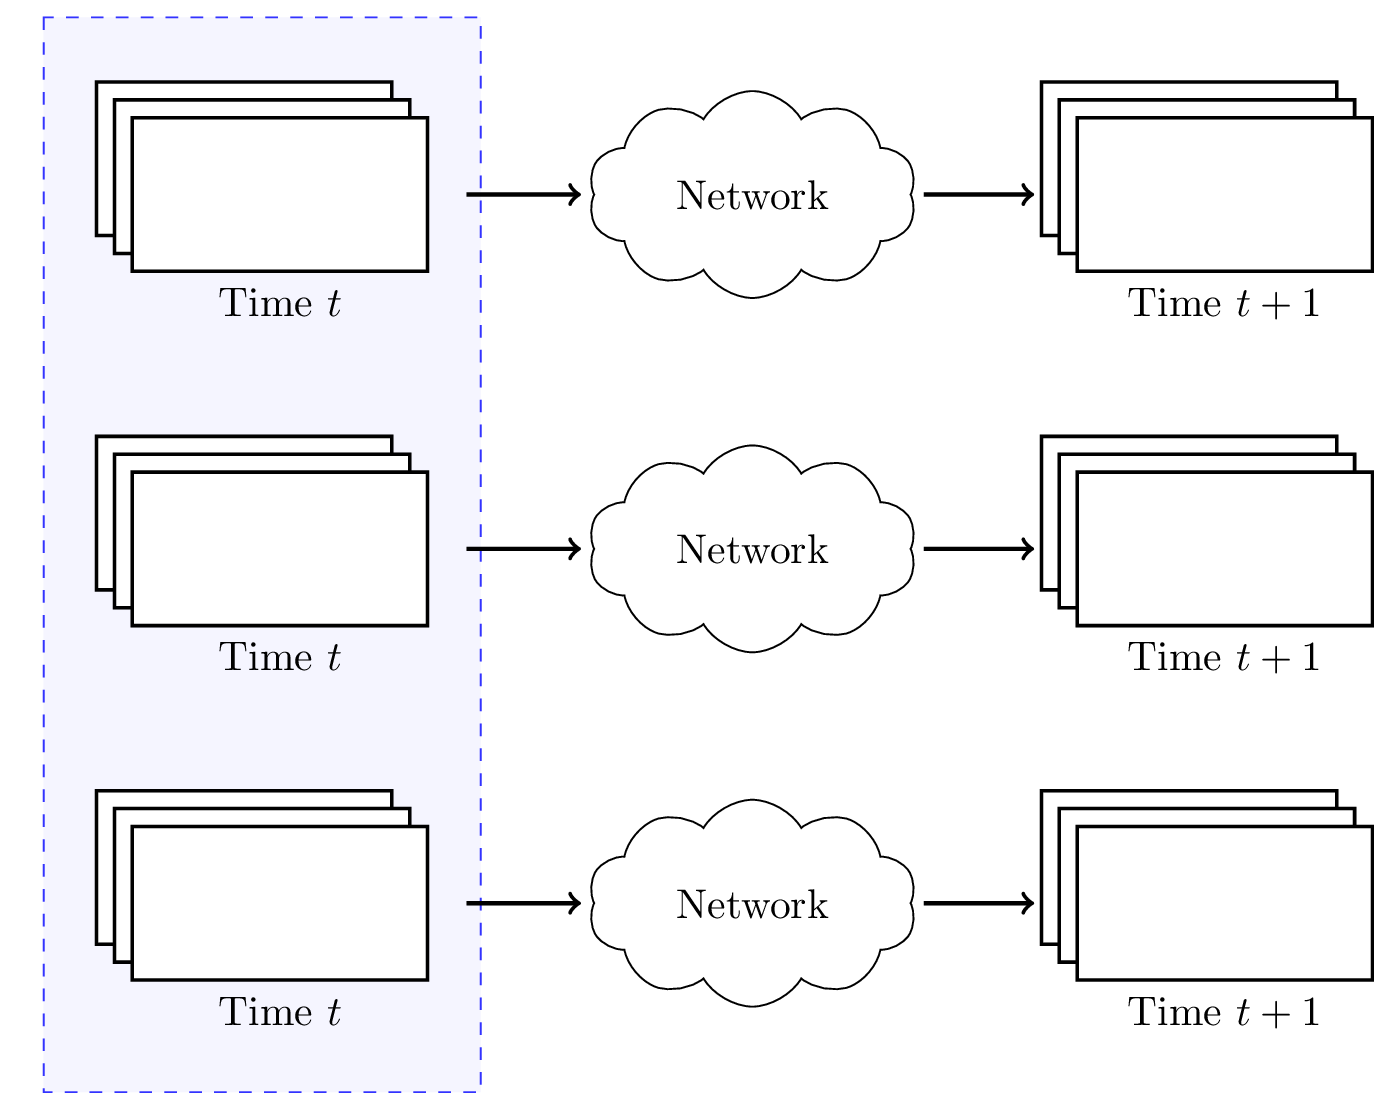
\includegraphics[scale=0.12]{images/simple_eval}
      \end{center}
    \end{column}
    \begin{column}{0.5\textwidth}
      \begin{center}
        {\large \underline{Recursive Application}}
        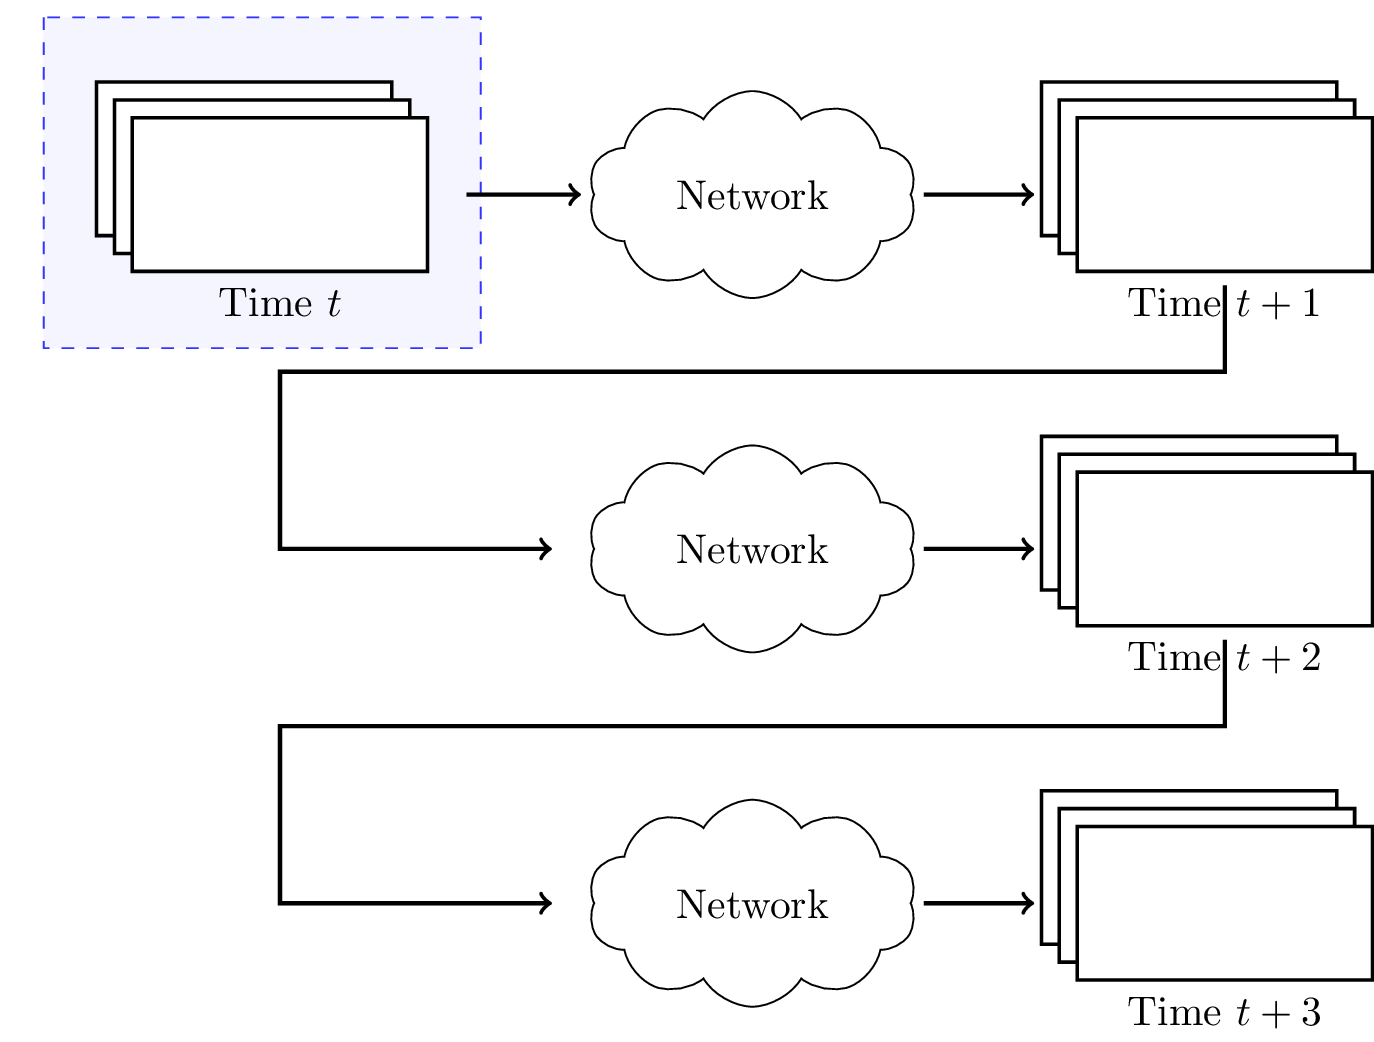
\includegraphics[scale=0.12]{images/rec_eval}
      \end{center}
    \end{column}
  \end{columns}
\end{frame}

\section{Results}
\begin{frame}[t]
  \frametitle{Results}
  \vspace{-1cm}
  \begin{center}
    {\large \underline{Individual Images -- constant model}} \\
    Cor. and PSNR:
  \end{center}
  \vspace{-1.3cm}
  \begin{columns}[t]
    \begin{column}{0.5\textwidth}
      \begin{center}
        \includegraphics[scale=0.22]{images/res/Models_PSNR}
      \end{center}
    \end{column}
    \begin{column}{0.5\textwidth}
      \begin{center}
        \includegraphics[scale=0.22]{images/res/Models_COR}
      \end{center}
    \end{column}
  \end{columns}
\end{frame}

\begin{frame}[t]
  \frametitle{Results}
  \vspace{-1cm}
  \begin{center}
    {\large \underline{Individual Images -- constant model}} \\
    Prediction image:
  \end{center}

  \begin{center}
    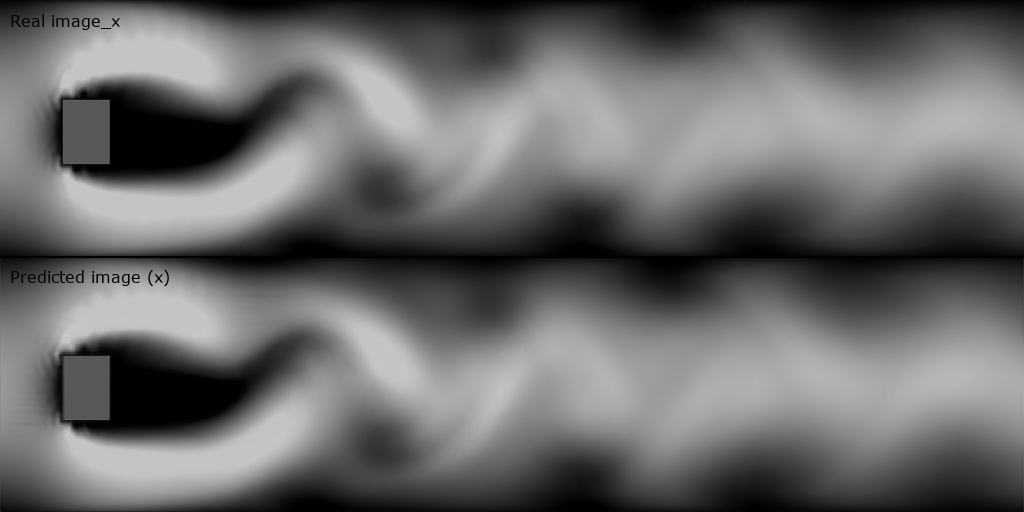
\includegraphics[scale=0.32]{images/res/prediction}
  \end{center}  
\end{frame}

\begin{frame}[t]
  \frametitle{Results}
  \vspace{-1cm}
  \begin{center}
    {\large \underline{Individual Images -- constant model}} \\
    Timestep image:
  \end{center}

  \begin{center}
    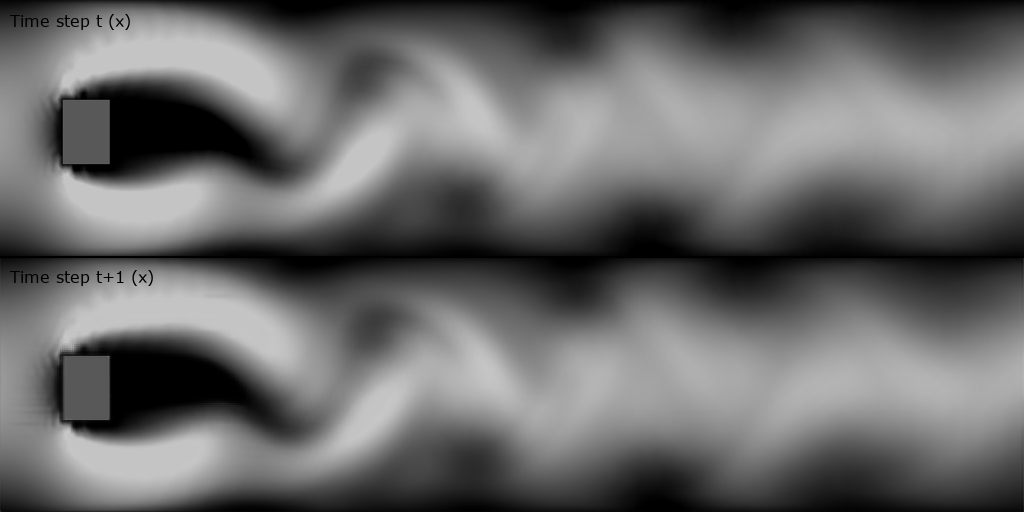
\includegraphics[scale=0.32]{images/res/timestep}
  \end{center}  
\end{frame}

\begin{frame}[t]
  \frametitle{Results}
  \vspace{-1cm}
  \begin{center}
    {\large \underline{Individual Images -- constant model}} \\
    Numerical view:
  \end{center}
  \vspace{-0.8cm}
  \begin{columns}[t]
    \begin{column}{0.5\textwidth}
      \begin{center}
        \textbf{Avrg difference} \\
        \includegraphics[scale=0.21]{images/res/Models_AVRG_DIFF}
      \end{center}
    \end{column}
    \begin{column}{0.5\textwidth}
      \begin{center}
        \textbf{Max difference} \\
        \includegraphics[scale=0.21]{images/res/Models_MAX_DIFF}
      \end{center}
    \end{column}
  \end{columns}
\end{frame}


\begin{frame}[t]
  \frametitle{Results}
  \vspace{-1cm}
  \begin{center}
    {\large \underline{Recursive application -- constant model}} \\
  \end{center}
  \begin{center}
    \includegraphics[scale=0.25]{images/res/rec_avrg}
  \end{center}
\end{frame}

\begin{frame}[t]
  \frametitle{Results}
  \vspace{-1cm}
  \begin{center}
    {\large \underline{Recursive application -- constant model}} \\
  \end{center}
  \vspace{1cm}
  \begin{center}
    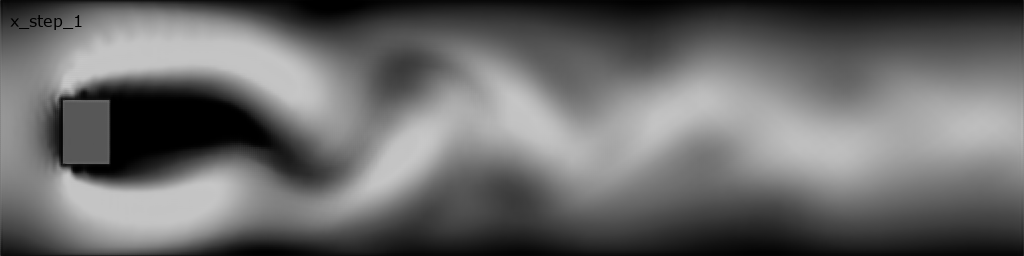
\includegraphics[scale=0.15]{images/res/x_step_1}
    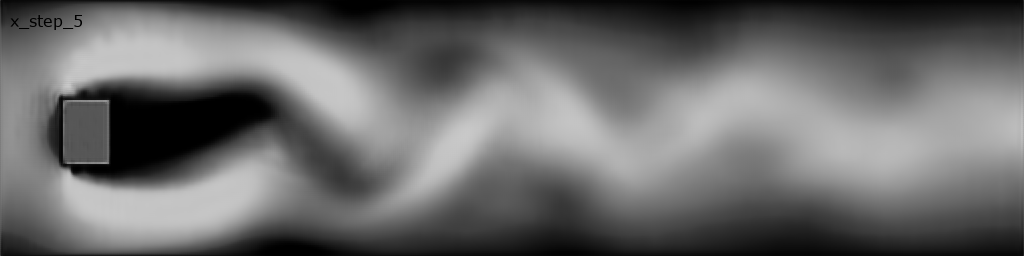
\includegraphics[scale=0.15]{images/res/x_step_5}
    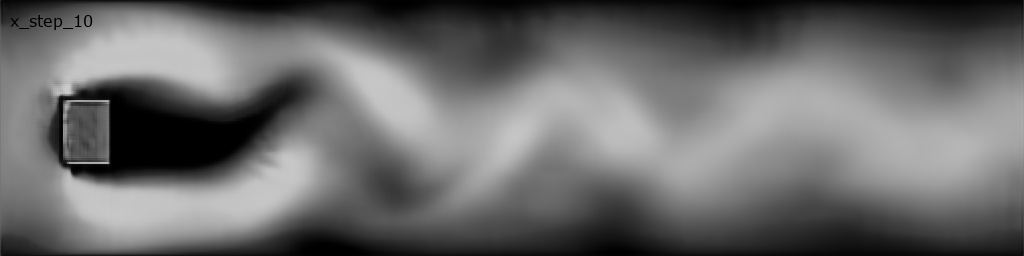
\includegraphics[scale=0.15]{images/res/x_step_10}
    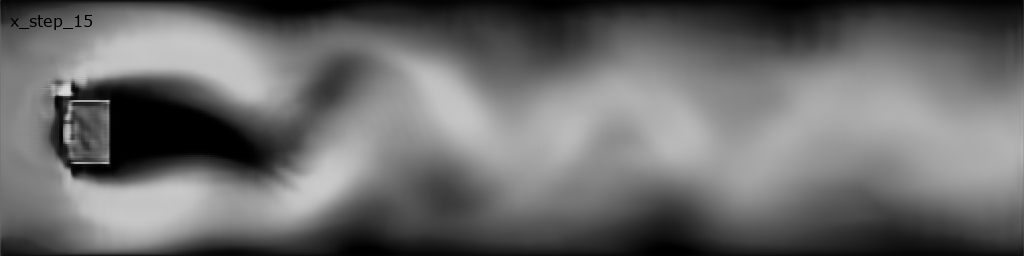
\includegraphics[scale=0.15]{images/res/x_step_15}
    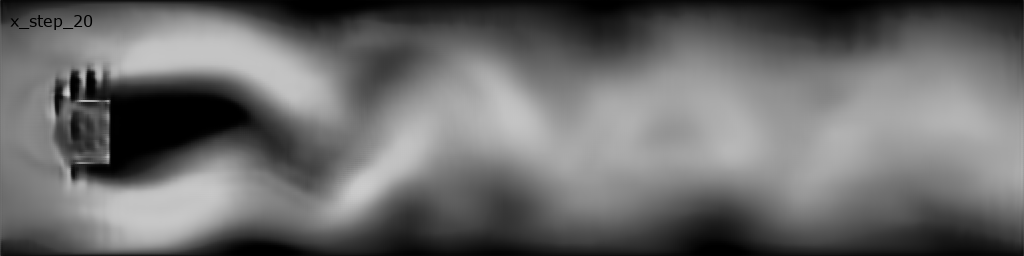
\includegraphics[scale=0.15]{images/res/x_step_20}
    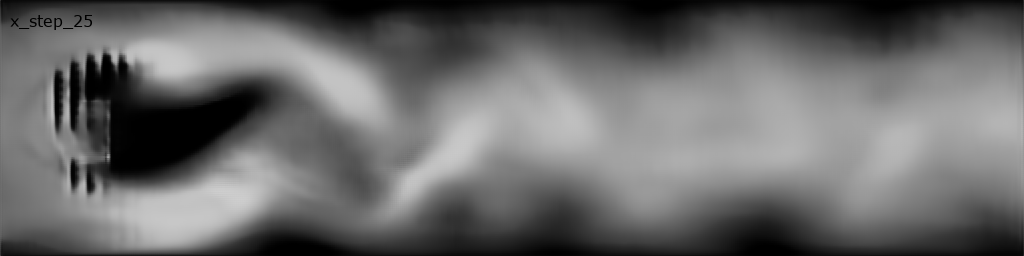
\includegraphics[scale=0.15]{images/res/x_step_25}
  \end{center}
\end{frame}


\section{End}
\begin{frame}
  \frametitle{}
  \begin{center}
    \huge{Thank you for your attention.}
  \end{center}
\end{frame}

\begin{frame}
  \frametitle{}
  \begin{center}
    \huge{Questions?}
  \end{center}
\end{frame}

\end{document}

%%% Local Variables:
%%% mode: latex
%%% TeX-master: t
%%% End:
